\section{What is a function?}
\begin{itemize}
    \item In C++ programs we typically make use of:
        \begin{itemize}
            \item C++ standard library (functions and classes).
            \item Third-party library (functions and classes).
            \item Our own functions and classes.
        \end{itemize}
    
    \item Functions allow the modularization of a program.
        \begin{itemize}
            \item Which allow us to separate code into logical self-contained units.
            \item These units can be reused.
        \end{itemize}
    
    \item Why we want to use functions?
        \begin{itemize}
            \item Which code is better?
        \end{itemize}
        \begin{center}
            \begin{tabular}{ |c|c| }
                \hline
                    Without functions & With functions \\
                \hline
                    \begin{minted}[autogobble]{cpp}
                        int main() {
                            // read input
                            statement1;
                            statement2;
                            statement3;
                            statement4;
                            // process input
                            statement5;
                            statement6;
                            statement7;
                            // provide input
                            statement8;
                            statement9;
                            statement10;
                            return 0;
                        }

                    \end{minted}
                    & 
                    \begin{minted}[autogobble]{cpp}
                        int main() {
                        // read input
                        read_input();
                        // process input
                        process_input();
                        // provide input
                        provide_input();
                        return 0;
                    }
                    \end{minted} \\ 
                \hline
            \end{tabular}
        \end{center}
        \begin{itemize}
            \item Functions allow for abstraction.
            \item Functions allow us to use the same code again and again and not having to be copying and pasting everything.
        \end{itemize}
    
    \item What is a function? The boss/worker analogy.
        \begin{itemize}
            \item Write your code to the function specification.
            \item Understand what the function does.
            \item Understand what information the function needs.
            \item Understand what the function returns.
            \item Understand any errors the function my produce.
            \item Understand any performance constraints.
            \item Don't worry about how the function works internally:
                \begin{itemize}
                    \item Unless you are the one writing the function.
                    \item This concept is called information hidding.
                \end{itemize}
        \end{itemize}
    
    \item Example: \mintinline{cpp}{<cmath>}
        \begin{itemize}
            \item Common mathematical calculations.
            \item Global functions called as:   
                \begin{itemize}
                    \item Global functions mean they are available to the entire program.
                \end{itemize}
                \begin{verbatim}
                    function_name(argument);
                    function_name(argument1, argument2, ...);
                \end{verbatim}
        \end{itemize}
    
    \item User defined functions:
        \begin{itemize}
            \item Implement only the functions you need, use the functions already implemented if posible.
            \item \url{https://en.cppreference.com/w/cpp/header} You can check functions.
        \end{itemize}
\end{itemize}

\subsection{Example}
\begin{itemize}
    \item Math:
        \begin{minted}[autogobble]{cpp}
            #include <iostream>
            #include <cmath>
            using namespace std;
            int main() {
                double num {12.5};
                cout << sqrt(num) << endl;
                return 0;
            }
            /* OUTPUT:
            3.53553
            */
        \end{minted}
\end{itemize}


%----------------------------------------------------------------------------------------
\section{Function definition}
Functions follow four main parts:
\begin{itemize}
    \item Functions perform operations.
    \item Once a function is defined you can call it from anywhere in the program. 
    \item Functions need to be declared before they are used.
\end{itemize}
\begin{itemize}
    \item Name: 
        \begin{itemize}
            \item The name of the function.
            \item Function names must be descriptive.
            \item Same rules as for variable names.
            \item Should be meaningful.
            \item Usually a verb or verb phrase.
        \end{itemize}
    
    \item Parameter list:
        \begin{itemize}
            \item The variables passed into the function.
            \item You can pass no variables.
            \item Their types must be specified.
        \end{itemize}
    
    \item Return type:
        \begin{itemize}
            \item The type of the data that is returned from the function.
            \item It's possible that the function does not return anything, in that case the type is \mintinline{cpp}{void}.
        \end{itemize}
    
    \item Body: 
        \begin{itemize}
            \item The statements that are executed when the function is called.
            \item In curly braces \{\}.
        \end{itemize}
\end{itemize}

\subsection{Example}
\begin{itemize}
    \item Example of function:
        \begin{minted}[autogobble]{cpp}
            int function_name(int a) {
                return a;
            }
        \end{minted}
    
    \item Example of area of the circle:
        \begin{minted}[autogobble]{cpp}
            #include <iostream>
            using namespace std;

            const double pi {3.4159};

            double calc_area_circle(double radious) {
                return pi * radious * radious;
            }

            void area_circle() {
                double radious {};
                cout << "Enter the radious of the circle: ";
                cin >> radious;

                cout << "The area of a circle with radious " << radious << " is " << calc_area_circle(radious) << endl;
            }

            double calc_volume_cylinder(double radious, double height) {
                return calc_area_circle(radious) * height;
            }

            void volume_cylinder() {
                double radious {};
                double height {};
                cout << "Enter the radious of the cylinder: ";
                cin >> radious;
                cout << "Enter the height of the cylinder: ";
                cin >> height;
                cout << "The volume of a cylinder with radious " << radious << " and height " << height << " is " << calc_volume_cylinder(radious, height) << endl;
            }

            int main() {
                area_circle();
                volume_cylinder();
                return 0;
            }
            /* OUTPUT:
            Enter the radious of the circle: 78
            The area of a circle with radious 78 is 20782.3
            Enter the radious of the cylinder: 78
            Enter the height of the cylinder: 90
            The volume of a cylinder with radious 78 and height 90 is 1.87041e+06

            */
        \end{minted}
\end{itemize}


%----------------------------------------------------------------------------------------
\section{Function prototypes}
\begin{itemize}
    \item The compiler must know about a function before it is used.
    \item This implies that either you define functions before calling them or you can use \emph{function prototypes.}
    \item Defining functions before they are called is OK for small programs, however not at all practical for larger programs.
    \item Using function prototypes allows us to define the functions anywhere in the code, because they are technically being 'declared' beforehand.
        \begin{itemize}
            \item Function prototypes tells the compiler what it needs to know without a full function definition.
            \item Also called ``forward declarations'' since you are telling the compiler how the function is going to look like and the compiler will enforce those rules.
            \item Function prototypes are placed at the beginning of a program.
            \item Also used in out own header files (.h). Functions defined in header files must contain their corresponding function prototypes in the same file.
        \end{itemize}
    
    \item Syntax of function prototype:
        \begin{verbatim}
            int function_name(); // prototype.
        
            int function_name() { // function definition.
                statement(s);
                return 0;
            }
        \end{verbatim}
    
    \item Function prototypes can include parameter names.
        \begin{verbatim}
            int function_name(int); // prototype with out names.
            int function_name(int a); // prototype with parameter names.
            int function_name(int a) {
                statement(s);
                return 0;
            }
        \end{verbatim}
    
    \item With \mintinline{cpp}{void} the return type is optional:
        \begin{verbatim}
            void function_name(); // prototype.
            void function_name() {
                statement(s);
                return; // optional
            }
        \end{verbatim}
    
    \item Function parameters help the compiler enforce the rules, for example what parameters it takes in, what types are those parameters, etcetera.
        \begin{minted}[autogobble]{cpp}
            #include <iostream>
            using namespace std;

            void say_hello();

            int main() {
                say_hello(); // OK
                say_hello(100); // error
                cout << say_hello(); // error, cout expects to print something and there is no return value
                return 0;
            }
            /* OUTPUT:

            */
        \end{minted}
\end{itemize}


%----------------------------------------------------------------------------------------
\section{Function parameters and the return statement}
\subsection{Function parameters}
\begin{itemize}
    \item Function parameters:
        \begin{itemize}
            \item When we call a function we can pass in data to that function.
            \item In the function call they are called arguments.
            \item In the function definition they are called parameters.
            \item They must match in number, order, and type.
        \end{itemize}
        \begin{minted}[autogobble]{cpp}
            #include <iostream>
            using namespace std;

            int add_numbers(int, int); // prototype.
                        
            int main() {
                int result {0};
                result = add_numbers(100,200); // call.
                cout << result << endl;
                return 0;
            }

            int add_numbers(int a, int b) { // function definition.
                return a + b;
            }

            /* OUTPUT:
            300
            */
        \end{minted}

    \item If the compiler knows how to convert a type it will convert.
        \begin{minted}[autogobble]{cpp}
            #include <iostream>
            using namespace std;

            void say_hello(string);

            void say_hello(string name) {
                cout << "Hello " << name << endl;
            }

            int main() {
                say_hello("C++"); // Sending a string literal not a std::string. The compiler will convert.
                return 0;
            }
            /* OUTPUT:
            Hello C++

            */
        \end{minted}
    
    \item Pass-by-value:
        \begin{itemize}
            \item When you pass data into a function it is passeded-by-value.
            \item A copy of the data is passed to the function.
            \item Whatever changes you make to the parameter in the function does NOT affect the argument that was passed in.
            \item This is good because the original data is not touched by the function if something goes wrong, and bad because sometimes copying the function parameters is expensive in terms of memory space, time and money. And sometimes you really do need to change the data that is passed in.
            \item Formal vs. Actual parameters:
                \begin{itemize}
                    \item Formal parameters: the parameters defined in the function header.
                    \item Actual parameters (arguments): the parameters used in the function call.
                \end{itemize}
            
            \item In C++ the actual parameters are passed by value or copied to the formal parameters.
        \end{itemize}
        \begin{minted}[autogobble]{cpp}
            #include <iostream>
            using namespace std;

            void param_test(int formal) { // formal is a copy if actual.
                cout << formal << endl; // 50
                formal = 100; // only changes the local (formal) copy.
                cout << formal << endl; // 100.
            }

            int main() {
                int actual {50}; 
                cout << actual << endl; // 50.
                param_test(actual); // pass in 50 to param_test.
                cout << actual << endl; // actual (50) did not change.
                return 0;
            }
            /* OUTPUT:
            50
            50
            100
            50

            */
        \end{minted}
\end{itemize}

\subsection{Function return statement}
\begin{itemize}
    \item If a function returns a value of a specific type then it must use a \mintinline{cpp}{return} statement that returns a value.
    \item If a function does not return a value (\mintinline{cpp}{void}) then the \mintinline{cpp}{return} statement is optional.
    \item \mintinline{cpp}{return} statement can occur anywhere in the body of the function, but it is usually used in the end of the function.
    \item \mintinline{cpp}{return} statement immediately exits the function.
    \item We can have multiple \mintinline{cpp}{return} statements in a function:
        \begin{itemize}
            \item Avoid many return statements in a function.
        \end{itemize}
    
    \item The return value is the result of the function call.
\end{itemize}


%----------------------------------------------------------------------------------------
\section{Default arguments}
\begin{itemize}
    \item When a function is called, all arguments must be supplied.
    \item Sometimes some of the arguments have the same values most of the time.
    \item We can tell the compiler to use default values if the arguments are not supplied.
    \item Default values can be in the prototype or definition, not both:
        \begin{itemize}
            \item Best practice is to have them in the prototype.
            \item Must appear at the tail end of the parameter list.
        \end{itemize}
    
    \item Can have multiple default values.
        \begin{itemize}
            \item Must appear consecutively at the tail end of the parameter list. 
        \end{itemize}
\end{itemize}

\subsection{Example}
\begin{itemize}
    \item Example:
        \begin{minted}[autogobble]{cpp}
            #include <iostream>
            using namespace std;

            double calc_cost(double base_cost, double tax_rate = 0.06);

            double calc_cost(double base_cost, double tax_rate) {
                return base_cost += (base_cost * tax_rate);
            }

            int main() {
                double cost {0};
                cost = calc_cost(200.0); // will use the default tax.
                cout << cost << endl;
                cost = calc_cost(100.0, 0.08); // will use 0.08 not the default
                cout << cost << endl;
                return 0;
            }
            /* OUTPUT:
            212
            108

            */
        \end{minted}
\end{itemize}


%----------------------------------------------------------------------------------------
\section{Overloading functions}
\begin{itemize}
    \item Sometimes we want to use a function to perform operations in several data types, such as the print function would need to admit any type of parameter.
    \item We can have functions that have different parameter lists that have the same name.
    \item This is a great example of abstraction, since we just think of ``print'' and not worry about the data type being passed in.  
    \item This is a type of polymorphism.
        \begin{itemize}
            \item We can have the same name work with different data types to execute similar behavior.
        \end{itemize}
    
    \item The compiler must be able to tell the functions apart based on the parameter list and argument supplied.
    \item All overloaded functions must be implemented separately, this could be solved with templates.
    \item If the function don't have any parameters and just vary on the return type a compiler error will be produced.
    \item The ease of use of overloading functions is just the abstraction, you can just think of a concept and not have to worry in which data type you implemented the function in, the compiler will deduce that for you.
    \item Be careful when using default values in more than one overloaded function, the compiler will not know which one to use, and this can cause a compiler error.
    \item Consider the following:
        \begin{minted}[autogobble]{cpp}
            #include <iostream>
            using namespace std;

            int add_numbers(int a, int b);
            double add_numbers(double a, double b);

            double add_numbers(double a, double b) {
                return a + b;
            }
            int add_numbers(int a, int b) {
                return a + b;
            }

            int main() {
                cout << add_numbers(10,20) << endl;
                cout << add_numbers(10.1,67.9) << endl;
                return 0;
            }
            /* OUTPUT:
            30
            78

            */
        \end{minted}
\end{itemize}

\subsection{Example}
\begin{minted}[autogobble]{cpp}
    #include <iostream>
    #include <vector>
    using namespace std;

    void print(int);
    void print(double);
    void print(string);
    void print(string, string);
    void print(vector<string>);

    void print(int num) {
        cout << "int:" << num << endl;
    }
    void print(double num) {
        cout << "double: " << num << endl;
    }
    void print(string str) {
        cout << "string: " << str << endl;
    }
    void print(string str1, string str2) {
        cout << "str1: " << str1 << ", str2: " << str2 << endl;
    }
    void print(vector<string> vec) {
        for (auto v : vec) {
            cout << v << endl;
        }
    }

    int main() {
        print(100); // int -> print(int)
        print('A'); // char -> print(int) char is promoted to int.
        print(123.5); // double -> print(double)
        print(123.3F); // float -> print(double) float is promoted to double.
        print("C-style string"); // C-style string is converted to a C++ string.
        vector<string> vec {"ABC", "DEF", "GHI"};
        print(vec);
        return 0;
    }
    /* OUTPUT:
    int:100
    int:65
    double: 123.5
    double: 123.3
    string: C-style string
    ABC
    DEF
    GHI

    */
\end{minted}


%----------------------------------------------------------------------------------------
\section{Passing arrays to functions}
\begin{itemize}
    \item We can pass an array to a function by providing square brackets in the formal parameter description.
        \begin{verbatim}
            void print_array(int numbers[]);
        \end{verbatim}
    
    \item The array elements are NOT copied, the function does not know how many times to iterate through the array because what is passed in is an address to the array not a copy of the array.
    \item Since the array name evaluates to the location of the array in memory, this address is what is copied.
    \item So the function has no idea how many elements are in the array since all it knows is the location of the first element (the name of the array).
    \item So when we pass arrays to functions we must also pass in the size of the array in order to know how much time to iterate.
    \item Example:
        \begin{minted}[autogobble]{cpp}
            #include <iostream>
            using namespace std;

            void print_array(int numbers[], size_t size);

            int main() {
                int my_numbers[] {1,2,3,4,5};
                print_array(my_numbers, 5);
                return 0;
            }

            void print_array(int numbers[], size_t size) {
                for (size_t i{0}; i < size; ++i) {
                    cout << numbers[i] << endl;
                }
            }
            /* OUTPUT:
            1
            2
            3
            4
            5

            */
        \end{minted}
    
    \item In this case since the array is not copied but instead C++ works with the original array, we sometimes don't want to risk changing or altering the array passed in. Since we are passing the location of the array the function can modify the actual array.
        \begin{itemize}
            \item For this we can tell the compiler that function parameters are \mintinline{cpp}{const} (read-only).
            \item This could me useful in the \mintinline{cpp}{print_array} function since if should NOT modify the array.
        \end{itemize}
        \begin{minted}[autogobble]{cpp}
            void print_array(const int numbers[], size_t size) {
                for (size_t i{0}; i < size; ++i) {
                    cout << numbers[i] << endl;
                }
            }
        \end{minted}
\end{itemize}


%----------------------------------------------------------------------------------------
\section{Pass by reference}
\begin{itemize}
    \item Sometimes we want to be able to change the actual parameter from within the function body.
    \item In order to achieve this we need the location or address of the actual parameter.
    \item We say how this is the effect with array, but what about other variable types?
    \item We can use reference parameters to tell the compiler to pass in a reference to the actual parameter.
    \item The formal parameter will now be an alias for the actual parameter.
    \item Syntax is: \verb|return_type func_name(type &var_name);|
    
    \item Example:
        \begin{minted}[autogobble]{cpp}
            #include <iostream>
            using namespace std;

            void scale_number(int &num);

            int main() {
                int number {1000};
                scale_number(number);
                cout << number << endl;
                return 0;
            }

            void scale_number(int &num) {
                if (num > 100) {
                    num = 100;
                }
            }

            /* OUTPUT:
            100

            */
        \end{minted}
    
    \item Example:
        \begin{minted}[autogobble]{cpp}
            #include <iostream>
            using namespace std;

            void swap(int &a, int &b) {
                int temp = a;
                a = b;
                b = temp;
            }

            int main() {
                int x{10}, y{20};
                cout << x << " " << y << endl;
                swap(x,y);
                cout << x << " " << y << endl;
                return 0;
            }
            /* OUTPUT:
            10 20
            20 10

            */
        \end{minted}
    
    \item In the following we intend to pass a vector by value in to the function print which would mean that it will make a copy of all that data inside the function. We could better pass the location of the vector into the function and modify the original data:
        \begin{itemize}
            \item The issue now would be that we could pass by reference and risk modifying the vector in an unintended way, for this we can make the data being passed in constant.
            \item This is the best of both worlds because we are passing the reference (which is more efficient) and at the same time ensuring no changes are made to the vector.
        \end{itemize}
        \begin{minted}[autogobble]{cpp}
            #include <iostream>
            #include <vector>
            using namespace std;

            void print(const vector<int> &v) {
                for (auto num : v) {
                    cout << num << endl;
                }
            }

            int main() {
                vector<int> data {1,2,3,4};
                print(data);
                return 0;
            }
            /* OUTPUT:
            1
            2
            3
            4

            */
        \end{minted}
\end{itemize}


%----------------------------------------------------------------------------------------
\section{Scope rules}
\begin{itemize}
    \item C++ uses scope rules to determine where an identifier can be used.
    \item C++ uses static or lexical scoping.
    \item C++ has two main scopes: Local or block scope:
        \begin{itemize}
            \item Local or block scopes:
                \begin{itemize}
                    \item Identifiers declared in a block \{\}.
                    \item Function parameters have block scope.
                    \item Only visible within the block \{\} where declared.
                    \item Function local variables are only active while the function is executing.
                    \item Local variables are not preserved between function calls.
                    \item With nested blocks inner blocks can 'see' but outer blocks cannot.
                    \item When a function is called you can think of the function as being activated and the function parameters are bound to storage. The parameters become alive and the their lifetime is the time the function executes, once the function completes the function is deactivated and these variables and parameters are no longer alive.
                \end{itemize}
        \end{itemize}
    
    \item Static local variables:
        \begin{itemize}
            \item There is one kind of variable whose value is preserved between many function calls.
                \begin{minted}[autogobble]{cpp}
                    static int value {10};
                \end{minted}
            \item It is a variable whose lifetime is the lifetime of the program.
            \item It is only visible to the statements in the function body.
            \item These variables can be very helpful when you need some values to be preserved in a function without having to pass them in each time.
            \item Static local variables are only initialized once, if no initialization is provided they are set to 0.
        \end{itemize}

    \item Identifiers with global scope.
        \begin{itemize}
            \item Identifiers declared outside any function or class.
            \item Visible to all parts of the program after the  global identifier has been declared.
            \item Global constants are OK.
            \item Best practice is not to use global variables.
        \end{itemize}
    
    \item You can create a new scope with the \{\}.
        \begin{minted}[autogobble]{cpp}
            #include <iostream>
            using namespace std;
            int main() {
                int num1 {100}; // local to main.
                int num2 {500}; // local to main.
                cout << "num1: " << num1 << " {" << endl;
                {
                    int num1 {200};
                    cout << "\tnum1: " << num1 << endl;
                    cout << "\tnum2: " << num2 << endl;
                }
                cout << '}' << endl;
                return 0;
            }
            /* OUTPUT:
            num1: 100 {
                    num1: 200
                    num2: 500
            }

            */
        \end{minted}
    
    \item One particular block can see outwardly while the out most blocks cannot see in to the most nested blocks.
\end{itemize}


%----------------------------------------------------------------------------------------
\section{How do function calls work?}
\begin{itemize}
    \item Functions use an area in memory called the function call stack:
        \begin{itemize}
            \item Analogous to a stack of books.
            \item Operations on a stack push and pop.
            \item In a program a push element in to the call stack is called a stack frame.
        \end{itemize}
    
    \item Stack frame or activation record:
        \begin{itemize}
            \item Functions must return control to function that called it.
            \item Each time a function is called we create an new activation record and push it on to the stack.
            \item When a function terminates we pop the activation record and return.
            \item Local variables and function parameters are located on the stack.
        \end{itemize}
    
    \item The stack size if finite:
        \begin{itemize}
            \item If you call too many functions you might run out of stack space producing a stack overflow error which will crash your program.
        \end{itemize}
    
    \item Illustration:
        \begin{figure}[H]
            \centering
            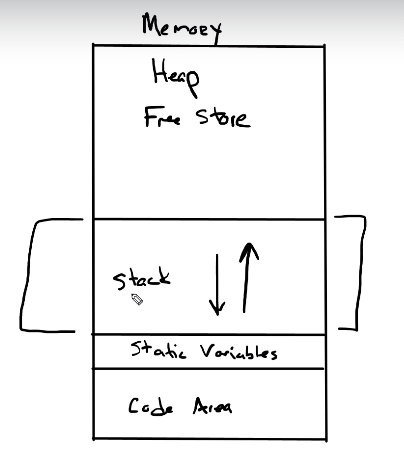
\includegraphics[width=0.4\textwidth]{./figs/funcall.png}
        \end{figure}
\end{itemize}


%----------------------------------------------------------------------------------------
\section{Inline functions}
\begin{itemize}
    \item As we've seen, a function requires space in the call stack, the creation of a stack frame and the deletion of the stack frame once the function is done.
    \item Sometimes the function is so simple the process a function has to undergo to become a function in memory is ineficient and not worth the code.
    \item Function calls have certaing amount of overhead.
    \item You saw what happens on the call stack.
    \item Sometimes we have simple functions.
    \item We can suggest to the compiler to compile them 'inline':
        \begin{itemize}
            \item Avoid function call overhead.
            \item Generate inline assembly code.
            \item Faster.
            \item Could cause code bloat.
        \end{itemize}
    
    \item Compilers optimizations are very sophisticated:
        \begin{itemize}
            \item Will likely make simple functions inline even without your suggestion.
        \end{itemize}
    
    \item Syntax is:
        \begin{minted}[autogobble]{cpp}
            inline int add_numbers(int a, int b) {
                return a + b;
            }
            int main() {
                int result{0};
                result = add_numbers(100,200);
                return 0;
            }
        \end{minted}
\end{itemize}


%----------------------------------------------------------------------------------------
\section{Recursive functions}
\begin{itemize}
    \item A recursive function is a function that calls itself.
        \begin{itemize}
            \item Either directly or indirectly through another function.
        \end{itemize}
    
    \item Recursive problem-solving:
        \begin{itemize}
            \item Base case.
            \item Divide the rest of the problem into subproblems and do a recursive call.
        \end{itemize}
    
    \item There are many problems that lend themselves to recursive solutions.
    \item Mathematics: factorial, Fibbonacci, fractals.
    \item Searching and sorting: binary search, search trees, ....
    \item Example of Factorial:
        \begin{align*}
            n! = n \times (n - 1);
        \end{align*}
        \begin{minted}[autogobble]{cpp}
            #include <iostream>
            using namespace std;
            unsigned long long factorial(unsigned long long n) {
                if (n == 0) {
                    return 1; // base case.
                }
                return n * factorial(n-1); // recursive call.
            }
            int main() {
                cout << factorial(8) << endl;
                return 0;
            }
            /* OUTPUT:
            40320

            */
        \end{minted}
    
    \item Important notes:
        \begin{itemize}
            \item If recursion doesn't eventually stop you will have infinite recursion.
            \item Recursion can be resource intensive (take up too much memory).
            \item Remember the base case(s):
                \begin{itemize}
                    \item It terminates the recursion.
                \end{itemize}
            
            \item Only use recursive solutions when it makes sense.
            \item Anything that can be done recursively can be done iteratively.
                \begin{itemize}
                    \item Stack overflow error.
                \end{itemize}
        \end{itemize}
\end{itemize}
